\documentclass[12pt, letterpaper, twoside]{article}
\usepackage[T1]{fontenc}
\usepackage[utf8]{inputenc}
\usepackage[russian]{babel}
\usepackage[a1paper]{geometry}
\geometry{papersize={29.7 cm, 25.0 cm}}
\usepackage{graphicx}
\title{DIFFERENCIATOR MACHINE}
\author{Makson from 225}
\date{}
\begin{document}
\maketitle
\newpage
\begin{center}
Your function is $F = x^{2} \cdot 6 \cdot x$\newline 
\begin{figure}
\begin{center}
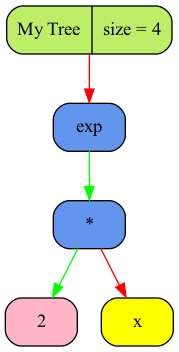
\includegraphics [scale = 0.4]{graphics/graph1.png}
\caption{Get your funtion}
\end{center}
\end{figure}
\end{center}
\newpage
Your function is $F = x^{2} \cdot 6 \cdot x$.
The value of your function at 3: $ F(3) = 162 $
\end{document}